\documentclass[xcolor=dvipsnames,12pt,aspectratio=169]{beamer}
\usecolortheme[named=violet]{structure} 

%\usetheme{umbc2} 
\usepackage{pgf}
%\usepackage[pdftex]{graphicx}
\usepackage{color}
\usepackage{amssymb,amsmath}
\usepackage[english]{babel}
\mode<presentation>

 \usepackage{multimedia}
\usefonttheme{structurebold}

%\useinnertheme{umbcboxes}

%\setbeamercolor{umbcboxes}{bg=violet!15,fg=black}  

\setbeamercovered{transparent}
\setbeamertemplate{navigation symbols}{}

%
%
% Adjustable parenthesis et al
%
\newcommand{\K}[1]{\left({#1}\right)}
\newcommand{\lp}{\left(}
\newcommand{\rp}{\right)}
\newcommand{\lb}{\left[}
\newcommand{\rb}{\right]}
\newcommand{\lc}{\left\{}
\newcommand{\rc}{\right\}}
\newcommand{\la}{\left\langle}
\newcommand{\ra}{\right\rangle}
\newcommand{\Dp}[3]{\langle #1,#2 \rangle_{#3}}
\newcommand{\cov}[2]{\langle #1\,#2 \rangle}

\newcommand{\half}{\mbox{$\frac{1}{2}$}} %

\newcommand{\U}{{\cal U}}
\newcommand{\C}{{\cal C}}
\newcommand{\X}{{\cal X}}
\newcommand{\Y}{{\cal Y}}

\newcommand {\ared} {{\rm ared}}
\newcommand {\pred} {{\rm pred}}
\newcommand {\rpred} {{\rm rpred}}

\newcommand{\sn}{s^{\sf n}}  % Normal component
\newcommand{\st}{s^{\sf t}}  % Tangential component
\newcommand{\rt}{r^{\sf t}}  % Tangential component
\newcommand{\stepy}{{s_y}}  % step in y--component
\newcommand{\stepu}{{s_u}}  % step in u--component

%
\newcommand{\veps}{{\varepsilon}} 
% Bolds and scripts
%
\newcommand{\CG}{\ensuremath{\mathcal{G}} }
\newcommand{\CQ}{\ensuremath{\mathcal{Q}} } %
\newcommand{\CR}{\ensuremath{\mathcal{R}} } %
\newcommand{\CW}{\ensuremath{\mathcal{W}} } %
\newcommand{\CX}{\ensuremath{\mathcal{X}} } %
\newcommand{\CZ}{\ensuremath{\mathcal{Z}} } %
\newcommand{\CU}{\ensuremath{\mathcal U} }
\newcommand{\CC}{\ensuremath{\mathcal C} }
\newcommand{\CD}{\ensuremath{\mathcal D} }
\newcommand{\BA}{\ensuremath{\mathbf{A}} } %
\newcommand{\BB}{\ensuremath{\mathbf{B}} } %
\newcommand{\BC}{\ensuremath{\mathbf{C}} } %
\newcommand{\BhC}{\ensuremath{\widehat{\mathbf{C}}} } %
\newcommand{\BD}{\ensuremath{\mathbf{D}} } %
\newcommand{\BE}{\ensuremath{\mathbf{E}} } %
\newcommand{\BF}{\ensuremath{\mathbf{F}} } %
\newcommand{\BG}{\ensuremath{\mathbf{G}} } %
\newcommand{\BH}{\ensuremath{\mathbf{H}} } %
\newcommand{\BK}{\ensuremath{\mathbf{K}} } %
\newcommand{\BL}{\ensuremath{\mathbf{L}} } %
\newcommand{\BM}{\ensuremath{\mathbf{M}} } %
\newcommand{\BN}{\ensuremath{\mathbf{N}} } %
\newcommand{\BP}{\ensuremath{\mathbf{P}} } %
\newcommand{\BQ}{\ensuremath{\mathbf{Q}} } %
\newcommand{\BR}{\ensuremath{\mathbf{R}} } %
\newcommand{\BU}{\ensuremath{\mathbf{U}} } %
\newcommand{\BW}{\ensuremath{\mathbf{W}} } %
\newcommand{\BX}{\ensuremath{\mathbf{X}} } %
\newcommand{\BY}{\ensuremath{\mathbf{Y}} } %
\newcommand{\BZ}{\ensuremath{\mathbf{Z}} } %
\newcommand{\ba}{\ensuremath{\mathbf{a}}}
\newcommand{\bb}{\ensuremath{\mathbf{b}}}
\newcommand{\bc}{\ensuremath{\mathbf{c}}}
\newcommand{\be}{\ensuremath{\mathbf{e}}}
\newcommand{\bg}{\ensuremath{\mathbf{g}}} %
\newcommand{\bh}{\ensuremath{\mathbf{h}}} %
\newcommand{\bk}{\ensuremath{\mathbf{k}}} %
\newcommand{\bn}{\ensuremath{\mathbf{n}}} %
\newcommand{\bp}{\ensuremath{\mathbf{p}}} %
\newcommand{\bq}{\ensuremath{\mathbf{q}}}
\newcommand{\br}{\ensuremath{\mathbf{r}}} %
\newcommand{\bs}{\ensuremath{\mathbf{s}}} %
\newcommand{\bt}{\ensuremath{\mathbf{t}}} %
\newcommand{\bu}{\ensuremath{\mathbf{u}}} %
\newcommand{\bv}{\ensuremath{\mathbf{v}}} %
\newcommand{\bdv}{\ensuremath{\mathbf{\delta v}}} %
\newcommand{\bw}{\ensuremath{\mathbf{w}}} %
\newcommand{\bd}{\ensuremath{\mathbf{d}}} %
\newcommand{\bx}{\ensuremath{\mathbf{x}}} %
\newcommand{\by}{\ensuremath{\mathbf{y}}} %
\newcommand{\obx}{\ensuremath{\overline{\mathbf{x}}}} %
\newcommand{\oby}{\ensuremath{\overline{\mathbf{y}}}} %
\newcommand{\obz}{\ensuremath{\overline{\mathbf{z}}}} %
\newcommand{\obw}{\ensuremath{\overline{\mathbf{w}}}} %
\newcommand{\bz}{\ensuremath{\mathbf{z}}} %
\newcommand{\blambda}{\mbox{\boldmath $\lambda$}}
\newcommand{\bdelta}{\mbox{\boldmath $\delta$}}
\newcommand{\bxi}{\mbox{\boldmath{$\xi$}}}
\newcommand{\bfeta}{\mbox{\boldmath $\eta$}}
\newcommand{\bkappa}{\mbox{\boldmath $\kappa$}}
\newcommand{\bmu}{\mbox{\boldmath $\mu$}}
\newcommand{\brho}{\mbox{\boldmath $\rho$}}
\newcommand{\bsigma}{\mbox{\boldmath $\sigma$}}
\newcommand{\sbxi}{\mbox{\scriptsize \boldmath{$\xi$}}}
\newcommand{\sbfeta}{\mbox{\scriptsize \boldmath $\eta$}}
\newcommand{\teta}{\mbox{\tiny \boldmath $\eta$}}
\newcommand{\txi}{\mbox{\tiny \boldmath{$\xi$}}}
\newcommand{\bLambda}{\mbox{\boldmath $\Lambda$}}
\newcommand{\bDelta}{\mbox{\boldmath $\Delta$}}
\newcommand{\bzero}{\mbox{\boldmath $0$}}
\newcommand{\bone}{\mbox{\boldmath $1$}}
\newcommand{\sDelta}{\mbox{\small $\Delta$}}
\newcommand{\tDelta}{\mbox{\tiny $\Delta$}}

\newcommand{\pd}[2]{\frac{\partial #1}{\partial #2}}
\newcommand{\ppd}[3]{\frac{\partial^{#3} #1}{\partial {#2}^{#3}}}
\newcommand{\pdsec}[3]{\frac{\partial^2 #1}{\partial #2\partial #3}}

\def\frechet{Fr\'echet\ }
%\newcommand{\real}{\mathbb{R}}
\newcommand{\real} {I\!\!R}
\newcommand{\nat} {{I\!\!N}}
\newcommand{\compl} {C\!\!\!\!I\;}
%
\def\Pr{\sf Pr}
\def\Re{\sf Re}
\def\M{{\sf M}}
\def\d{\delta}
\newcommand{\deq}{\raisebox{0pt}[1ex][0pt]{$\stackrel{\scriptscriptstyle{\rm def}}{{}={}}$}}
\newcommand{\dif}{{\mathrm d}}

\newcommand{\eref}[1]{\mbox{\rm(\ref{#1})}}
\newcommand{\tref}[1]{\mbox{\rm\ref{#1}}}


%\newenvironment{proof}{\noindent {\bf Proof:} }{\hfill $\Box$ \\[2ex] }

\newcommand{\myint}[1]{\int_0^T \dif t~{#1}}
\newcommand{\myintt}[1]{\int_0^1 \dif s~{#1}}
\newcommand{\dint}[1]{\int\limits_{#1}\!\!\!\int}

\newcommand{\waveop}[1]{c^{-2}{#1}_{tt}-\Delta{#1}}
\newcommand{\redwaveop}[1]{\Delta{#1}+k^2n^2{#1}}

\newcommand{\D}{\displaystyle}
%\allowdisplaybreaks
%

\setlength{\parskip}{2ex}   % place a blank line between paragraphs
\def\Logo{\@ifnextchar(\beamer@Logo\logo}
\def\beamer@Logo(#1,#2){\logo}

\AtBeginSection[]{
{\setbeamertemplate{logo}{}
 \begin{frame}<beamer>
    \frametitle{Agenda}
    \tableofcontents[currentsection]
  \end{frame}
}
}
% Images
% Macros
\newcommand{\peq}{\,+\hspace{-0.15cm}=}
\newcommand{\bm}{\bar{m}}
\newcommand{\dm}{\delta m}
\newcommand{\dom}{\delta \bar{m}}
\newcommand{\doma}{\delta \bar{m}_{\alpha}}
\newcommand{\om}{\bar{m}}
\newcommand{\bH}{{\bf H}}
\newcommand{\bR}{{\bf R}}
\newcommand{\bcF}{{\bar{\cal F}}}
\newcommand{\cF}{{\cal F}}
\newcommand{\oF}{\bar{F}}
\newcommand{\odF}{\bar{F}^{\dagger}}
\newcommand{\oS}{\bar{S}}
\newcommand{\oM}{\bar{M}}
\newcommand{\Ja}{J_{\alpha}}
\newcommand{\Na}{N_{\alpha}}
\newcommand{\dd}{\delta d}
\newcommand{\ddl}{\delta d_{\alpha}}


\title[]{Extended Inversion: when it works, and why}
\author[]{William W. Symes}
\institute[]{Rice University}
\date{December 2020}

\begin{document}
\frame{
\titlepage
}

\begin{frame}\frametitle{How to Cycle-Skip, in one easy lesson}
\only<1>{
Single trace transmission in a fluid:

Point source at $\bx=\bx_s$ radiates with transient intensity $w(t)$ (``wavelet'')

Resulting pressure wave propagates to point receiver at $\bx=\bx_r$, offset $|\bx_r-\bx_s|=h$

Pressure trace predicted by linear acoustics:
\[
p(t) = \frac{1}{4\pi h}w(t-mh) = (F[m]w)(t)
\]
where $m =$ pressure wave slowness ($=1/v_p$), $F$ = modeling operator - linear in w, nonlinear in m
}
\only<2>{
Inverse problem: given pressure trace $d(t)$, wavelet $w(t)$, and offset $h$, find slowness $m$ so that
\[
F[m] w  \approx d
\]
Standard approach: turn it into an optimization - minimize over $m$ the {\em mean square error}
\[
\frac{1}{2}\int\,dt\, (F[m]w(t) -d(t))^2 = \frac{1}{2}\|F[m]w-d\|^2 = J_{\rm FWI}[m;w,d]
\]

= world's simplest FWI task
}
\only<3>{
Asymptotic transient-ness:

Mother wavelet $w_1$: $w_1(t)=0, |t|>1$ and $\int w_1^2 = 1$

Scaled wavelets $w_{\lambda} = \frac{1}{\sqrt{\lambda}}w_1(t/\lambda)$: $w_{\lambda}(t)=0, |t|>\lambda$ and $\int w_{\lambda}^2 = 1$

NB: if center frequency of $w_1 = \omega_1$, then center frequency of $w_{\lambda} = \omega_1/\lambda$

Theorem Uh-Oh: If $d = F[m_*]w_{\lambda}$ (noise-free transient data) and $|m-m_*| > 2\lambda/r$, then
\[
J_{\rm FWI}[m;w_{\lambda},d] = \|d\|^2, \,\, \nabla_m J_{\rm FWI}[m;w_{\lambda},d] = 0
\]
}
\only<4>{
$J_{\rm FWI}[m;w_{\lambda},d]$, $d=F[m_*]w_{\lambda}$, $w_{\lambda}$ = Ricker wavelet center frequency = $1/\lambda$, $m_*=0.4$ s/km, $h=1 km$
\begin{center}
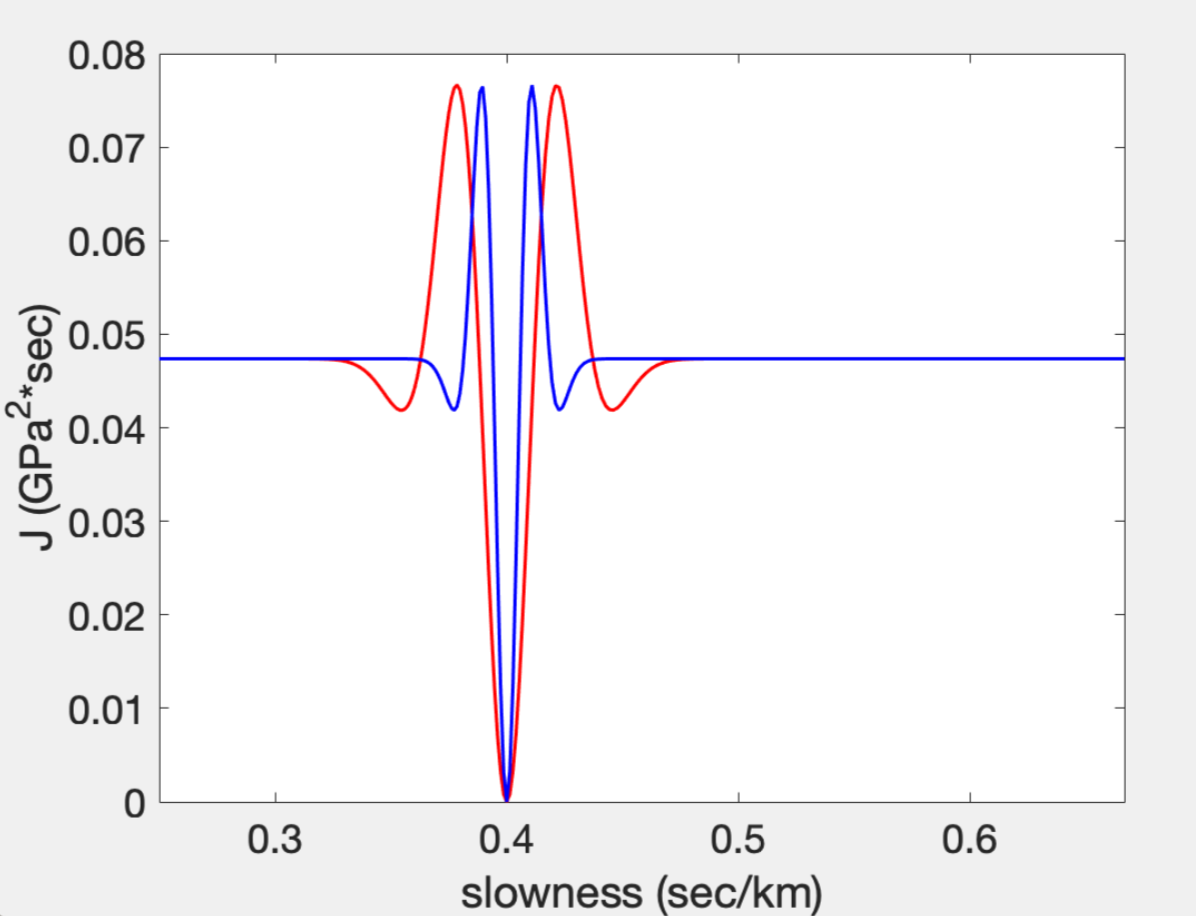
\includegraphics[height=4cm]{Fig/FWI.png}
\end{center}
Red: $\lambda=0.05$ (20 Hz), Blue: $\lambda = 0.25$ (40 Hz) [H. Chen et al. SEG 20]
}
\only<5>{
Postmortem:

\begin{itemize}
\item for most $m$, predicted data $F[m]w$ is not close to target data $d$
\item for most $m$, gradient is not a useful search direction
\item shape of objective function depends strongly on data frequency content - large residual, useless gradient more common for high frequencies (small $\lambda$)
\item flip side: low frequency (big $\lambda$) $\Rightarrow$ useful updates for larger set of initial models
\end{itemize}
}
\end{frame}

\begin{frame}\frametitle{Wavefield Reconstruction Inversion}
\only<1>{
Extended inversion: {\em enlarge the model space} = add (nonphysical) degrees of freedom, converge to point in original model space

WRI - van Leeuwen \& Herrmann GJI 13, IP 16, many other papers - most studied extended inversion approach

Idea: view wave equation as {\em weak constraint} $\sim$ {\em add source parameters}

Rationale: more likely to be able to 
\begin{itemize}
\item find low residual (extended) models (``hug your data''),
\item explore useful update directions
\end{itemize}
}
\only<2>{
Cast: 
\begin{itemize}
\item model parameters $m$ (eg. $m$=slowness)
\item Wave operator $L[m]$ (eg. constant density acoustic op
\[
\left. L[m]=m^2\frac{\partial^2}{\partial t^2} - \nabla^2\right)
\]
\item Known (!) source field $q(\bx,t)$ (eg. point source $w(t)\delta(\bx-\bx_s)$
\item dynamic fields $u(\bx,t)$ solve $L[m]u=q$ (eg. $u=$ pressure
\item Sampling operator $P$ extracts data trace(s) (pressure or ...) from $u$
\item Modeling operator $F[m]=PL[m]^{-1}$
\end{itemize}
}
\only<3>{
FWI: given $d$, $q$, 
\[
\min_m \|Pu-d\|^2 \mbox{ subj to } L[m]u=q
\]
\[
\Leftrightarrow \min_m \|F[m]q-d\|^2
\]

WRI: given $d$, $q$,
\[
\min_{m,u} \|Pu-d\|^2 + \alpha^2 \|L[m]u-q\|^2
\]

(NB: $\alpha$ small $\Rightarrow$ emphasis on 1st term $\Rightarrow$ ``hug your data'')
}
\only<4>{
equivalent (eg. Yingst \& Wang SEG 16): 

given $d$, $q$, set $g=L[m]u-q$, 

then $Pu-d = PL[m]^{-1}(g+q)-d = F[m]g + e[m]$ 

$e[m]=F[m]q-d$ = usual data residual

WRI: given $q,d$, 
\[
\min_{m,g} \|F[m]g+e[m]|^2 + \alpha^2 \|g|^2
\]
}
\only<5>{
Simplification 1:

Variable Projection (Golub \& Pereyra 73, 03): eliminate $g$ by solving quadratic minimization
\[
J_{\rm WRI}[m;q,d] = \min_{g} \|F[m]g+e[m]\|^2 + \alpha^2 \|g\|^2
\]
minimizer = $g[m;q,d]$, then
\[
=\|F[m]g[m;q,d]+e[m]|^2 + \alpha^2 \|g[m;q,d]\|^2
\]
$m$ minimizes $J_{\rm WRI}$ $\Leftrightarrow$ $(m,g[m;q,d])$ solves WRI problem 
}
\only<6>{
Simplification 2:

Non-radiating sources = $\{g: F[m]g=0\}$ = null space of $F[m]$

Rank-Nullity Theorem: $g = n + F[m]^Ts$, $s \in $ range of $F$ = data, $n$ = non-radiating, {\em and}
$n$ and $F[m]^Ts$ are orthogonal
\[
\|F[m]g+e[m]\|^2 + \alpha^2 \|g\|^2 = \|F[m](F[m]^Ts + n)+e[m]\|^2 + \alpha^2\|F[m]^Ts + n\|^2
\]
\[
= \|F[m]F[m]^Ts+e[m]\|^2 + \alpha^2\|F[m]^Ts\|^2 + \alpha^2\|n\|^2
\]
so
\[
J_{\rm WRI}[m;q,d] = \min_s \|F[m]F[m]^Ts-e[m]\|^2 + \alpha^2\|F[m]^Ts\|^2 
\]
}
\only<7>{
Simplification 3:

Minimization over $s$ $\Leftrightarrow$ solution of normal equation
\[
((F[m]F[m]^T)^2 + \alpha^2 F[m]F[m]^T)s = F[m]F[m]^Te[m]
\]
Substitute solution into def of $J_{\rm WRI}$, do a page of algebra (IP, v. 36 no. 10 (2020)), then...
\[
J_{\rm WRI} = \alpha^2 e[m]^T(F[m]F[m]^T + \alpha^2 I)^{-1} e[m]
\]
compare:
\[
J_{\rm FWI} = e[m]^T e[m]
\]
{\color{blue} $J_{\rm WRI}$ is weighted variant of $J_{\rm FWI}$, weight operator = $\alpha^2(F[m]F[m]^T + \alpha^2 I)^{-1} $}
}
\only<8>{
Apply to single-trace transmission:
\[
F[m]g(t) = \int_{r \le R}\,dx\,\frac{g(t-mr)}{4 \pi r}, \, F[m]^Ts(\bx,t) = 
\left\{\begin{array}{c}
\frac{s(t+mr)}{4 \pi r}, r\le R,\\
0, else
\end{array}
\right.
\]
($r = |\bx-\bx_r|$ and $g=0$ if $r > R$), so 
\[
F[m]F[m]^T s(t) = \frac{R}{4\pi} s(t),\,\,\alpha^2(F[m]F[m]^2 + \alpha^2 I)^{-1} =\frac{4\pi\alpha^2}{R + 4\pi\alpha^2}I
\]
}
\only<9>{
Theorem Uh-Oh \# 2:
\[
J_{\rm WRI}[m;w(t)\delta(\bx-\bx_s),d] = \frac{4\pi\alpha^2}{R + 4\pi\alpha^2} J_{\rm FWI}[m;w,d]
\]

Postmortem:
\begin{itemize}
\item WRI just as skippy as FWI!!!
\item enlarging the search space not enough
\item ``hugging your data'' also not enough: WRI cycle-skips for small $\alpha$
\item conclusion not limited to single trace transmission: similar for other transmission IPs, eg. diving wave inversion
\end{itemize}
}
\end{frame}

\begin{frame}\frametitle{Matched Source Extension}
\only<1>{
Back to FWI setting:
\[
F[m]w(t) = \frac{1}{4 \pi h}w(t-mh)
\]
A different extended inversion: add wavelet to unknowns

However, $F[m]$ is invertible for every $m$, so need constraint on $w$

Idea: after signature decon, wavelet should be {\em compact} $\sim$ nonzero only near $t=0$ - inspires {\em Matched Source Objective}
\[
\min_{m,w} \|F[m]w-d\|^2 + \|Aw\|^2, \,\,Aw(t)=tw(t)
\]
(S. 94, Plessix et al. 99, similar to Adaptive Waveform Inversion (AWI) Warner \& Guatsch 14)
}
\end{frame}
\end{document}


